\let\negmedspace\undefined
\let\negthickspace\undefined
\documentclass[journal,12pt,onecolumn]{IEEEtran}
\usepackage{cite}
\usepackage{amsmath,amssymb,amsfonts,amsthm}
\usepackage{algorithmic}
\usepackage{graphicx}
\graphicspath{{./figs/}}
\usepackage{textcomp}
\usepackage{xcolor}
\usepackage{txfonts}
\usepackage{listings}
\usepackage{enumitem}
\usepackage{mathtools}
\usepackage{gensymb}
\usepackage{comment}
\usepackage{caption}
\usepackage[breaklinks=true]{hyperref}
\usepackage{tkz-euclide} 
\usepackage{listings}
\usepackage{gvv}    
\usepackage{multicol}




\begin{document}
\title{
ASSIGNMENT 6: GATE 2024\\
GG : Geology and Geophysics}
\author{EE25BTECH11003 -Adharvan Kshathriya Bommagani}
\maketitle

\begin{enumerate}

\item If '$\rightarrow$' denotes increasing order of intensity, then the meaning of the words \brak{\text{simmer $\rightarrow$ seethe $\rightarrow$ smolder}} is analogous to \brak{\text{break $\rightarrow$ raze $\rightarrow$ \underline{\hspace{1.5cm}}}}. Which one of the given options is appropriate to fill the blank?

\hfill{\brak{\text{GATE GG 2024}}}

\begin{multicols}{4}
\begin{enumerate}
    \item obfuscate
    \item obliterate
    \item fracture
    \item fissure
\end{enumerate}
\end{multicols}

\item In a locality, the houses are numbered in the following way: The house-numbers on one side of a road are consecutive odd integers starting from 301, while the house-numbers on the other side of the road are consecutive even numbers starting from 302. The total number of houses is the same on both sides of the road. If the difference of the sum of the house-numbers between the two sides of the road is 27, then the number of houses on each side of the road is

\hfill{\brak{\text{GATE GG 2024}}}

\begin{multicols}{4}
\begin{enumerate}
    \item 27
    \item 52
    \item 54
    \item 26
\end{enumerate}
\end{multicols}

\item For positive integers $p$ and $q$, with $\frac{p}{q} \neq 1, \left(\frac{p}{q}\right)^{\frac{p}{q}} = p^{\left(\frac{p}{q}-1\right)}$. Then,

\hfill{\brak{\text{GATE GG 2024}}}

\begin{multicols}{2}
\begin{enumerate}
    \item $q^p = p^q$
    \item $q^p = p^{2q}$
    \item $\sqrt{q} = \sqrt{p}$
    \item $\sqrt[p]{q} = \sqrt[q]{p}$
\end{enumerate}
\end{multicols}

\item Which one of the given options is a possible value of x in the following sequence?
3, 7, 15, x, 63, 127, 255

\hfill{\brak{\text{GATE GG 2024}}}

\begin{multicols}{4}
\begin{enumerate}
    \item 35
    \item 40
    \item 45
    \item 31
\end{enumerate}
\end{multicols}

\item On a given day, how many times will the second-hand and the minute-hand of a clock cross each other during the clock time 12:05:00 hours to 12:55:00 hours?

\hfill{\brak{\text{GATE GG 2024}}}

\begin{multicols}{4}
\begin{enumerate}
    \item 51
    \item 49
    \item 50
    \item 55
\end{enumerate}
\end{multicols}




\item In the given text, the blanks are numbered (i)-(iv). Select the best match for all the blanks.
From the ancient Athenian arena to the modern Olympic \underline{\hspace{0.5cm}(i)\hspace{0.5cm}} stadiums, athletics \underline{\hspace{0.5cm}(ii)\hspace{0.5cm}} the potential for a spectacle. The crowd \underline{\hspace{0.5cm}(iii)\hspace{0.5cm}} with bated breath as the Olympian artist twists his body, stretching the javelin behind him. Twelve strides in, he begins to cross-step. Six cross-steps \underline{\hspace{0.5cm}(iv)\hspace{0.5cm}} in an abrupt stop on his left foot. As his body \underline{\hspace{0.5cm}(v)\hspace{0.5cm}} like a door turning on a hinge, the javelin is launched skyward at a precise angle.

\hfill{\brak{\text{GATE GG 2024}}}

\begin{enumerate}
    \item (i) hold (ii) waits (iii) culminates (iv) pivot
    \item (i) holds (ii) wait (iii) culminates (iv) pivot
    \item (i) hold (ii) wait (iii) culminate (iv) pivots
    \item (i) holds (ii) waits (iii) culminate (iv) pivots
\end{enumerate}

\item Three distinct sets of indistinguishable twins are to be seated at a circular table that has 8 identical chairs. Unique seating arrangements are defined by the relative positions of the people. How many unique seating arrangements are possible such that each person is sitting next to their twin?

\hfill{\brak{\text{GATE GG 2024}}}

\begin{multicols}{4}
\begin{enumerate}
    \item 12
    \item 14
    \item 10
    \item 28
\end{enumerate}
\end{multicols}

\item The chart given below compares the Installed Capacity (MW) of four power generation technologies, T1, T2, T3, and T4, and their Electricity Generation (MWh) in a time of 1000 hours (h). The Capacity Factor of a power generation technology is: $\frac{\text{Electricity Generation (MWh)}}{\text{Installed Capacity (MW)} \times 1000 \text{(h)}}$. Which technology has the highest Capacity Factor?

\begin{figure}[h!]
    \centering
    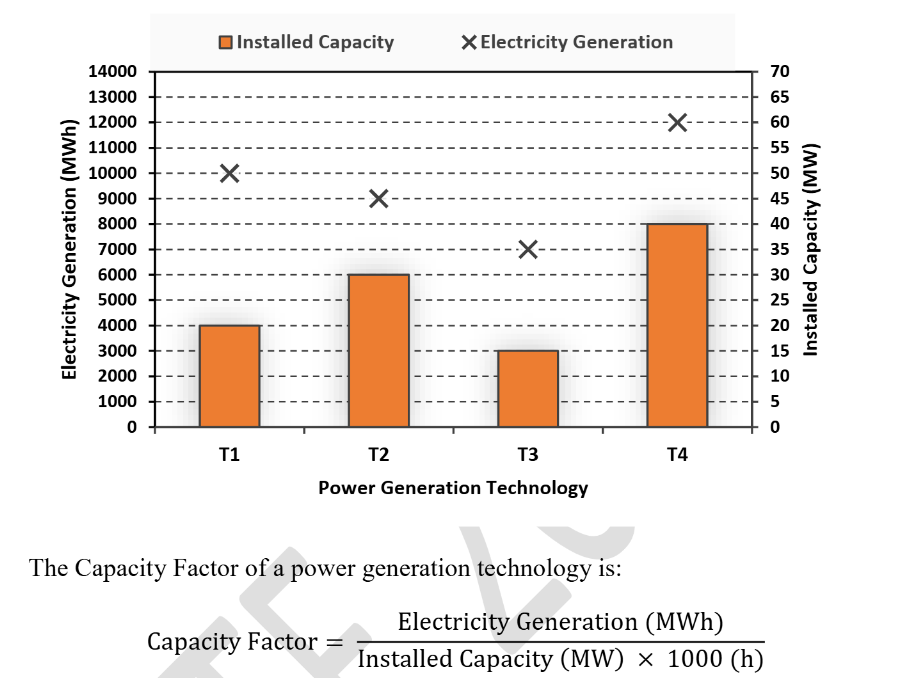
\includegraphics[width=0.4\textwidth]{figs/fig1.png}
    \caption{} 
    \label{fig:q18}
\end{figure}





\hfill{\brak{\text{GATE GG 2024}}}

\begin{multicols}{4}
\begin{enumerate}
    \item T1
    \item T2
    \item T3
    \item T4
\end{enumerate}
\end{multicols}

\item In the $4 \times 4$ array shown below, each cell of the first three columns has either a cross (X) or a number, as per the given rule. Rule: The number in a cell represents the count of crosses around its immediate neighboring cells (left, right, top, bottom, diagonals). As per this rule, the maximum number of crosses possible in the empty column is

\begin{figure}[h!]
    \centering
    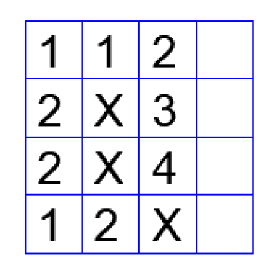
\includegraphics[width=0.4\textwidth]{figs/fig2.png}
    \caption{} 
    \label{fig:q18}
\end{figure}

\hfill{\brak{\text{GATE GG 2024}}}

\begin{multicols}{4}
\begin{enumerate}
    \item 0
    \item 1
    \item 2
    \item 3
\end{enumerate}
\end{multicols}

\item During a half-moon phase, the Earth-Moon-Sun form a right triangle. If the Moon-Earth-Sun angle at this half-moon phase is measured to be $89.85^{\degree}$, the ratio of the Earth-Sun and Earth-Moon distances is closest to

\hfill{\brak{\text{GATE GG 2024}}}

\begin{multicols}{4}
\begin{enumerate}
    \item 328
    \item 382
    \item 238
    \item 283
\end{enumerate}
\end{multicols}

\textbf{PART A: COMPULSARY SECTION FOR ALL CANDIDATES}




\item The Earth's magnetic field originates from convection in which one of the following layers?

\hfill{\brak{\text{GATE GG 2024}}}

\begin{multicols}{2}
\begin{enumerate}
    \item Inner core
    \item Outer core
    \item Lithosphere
    \item Asthenosphere
\end{enumerate}
\end{multicols}

\item Which one of the following logging tools is used to measure the diameter of a borehole?

\hfill{\brak{\text{GATE GG 2024}}}

\item The given figure depicts an array used in DC resistivity surveys, where the current electrodes are denoted by C1 and C2, and potential electrodes by P1 and P2. If all the electrodes are equally spaced, then the given array corresponds to which one of the following configurations?
\begin{figure}[h!]
    \centering
    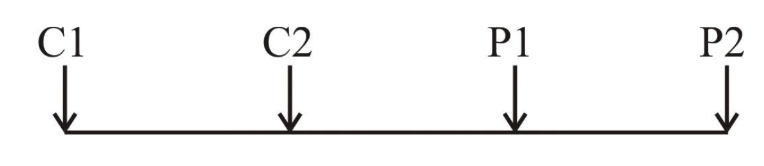
\includegraphics[width=0.4\textwidth]{figs/fig3.png}
    \caption{}
    \label{fig:q18}
\end{figure}



\hfill{\brak{\text{GATE GG 2024}}}

\begin{multicols}{2}
\begin{enumerate}
    \item Wenner
    \item Schlumberger
    \item Dipole-Dipole
    \item Pole-Pole
\end{enumerate}
\end{multicols}

\item Which one of the following is an ultramafic rock?

\hfill{\brak{\text{GATE GG 2024}}}

\begin{multicols}{4}
\begin{enumerate}
    \item Granite
    \item Gabbro
    \item Dunite
    \item Basalt
\end{enumerate}
\end{multicols}


\newpage

\item Gold is being produced from which one of the following mines in India?

\hfill{\brak{\text{GATE GG 2024}}}

\begin{multicols}{2}
\begin{enumerate}
    \item Baula
    \item Hutti
    \item Dariba
    \item Jaduguda
\end{enumerate}
\end{multicols}

\item Which of the following hydrocarbon fields is/are located in the western offshore of India?

\hfill{\brak{\text{GATE GG 2024}}}

\begin{multicols}{2}
\begin{enumerate}
    \item Tapti
    \item Lakwa
    \item Ravva
    \item Panna
\end{enumerate}
\end{multicols}

\item A cylindrical sample of granite \brak{\text{diameter = 54.7 mm; length = 137 mm}} shows a linear relationship between axial stress and axial strain under uniaxial compression up to the peak stress level at which the specimen fails. If the uniaxial compressive strength of this sample is 200 MPa and the axial strain corresponding to this peak stress is 0.005, the Young’s modulus of the sample in GPa is \underline{\hspace{1.5cm}} \brak{\text{in integer}}.

\hfill{\brak{\text{GATE GG 2024}}}




\item The given figure shows the ray path of a P–wave propagating through the Earth. Choose the CORRECT P–phase corresponding to the ray path.

\begin{figure}[h!]
    \centering
    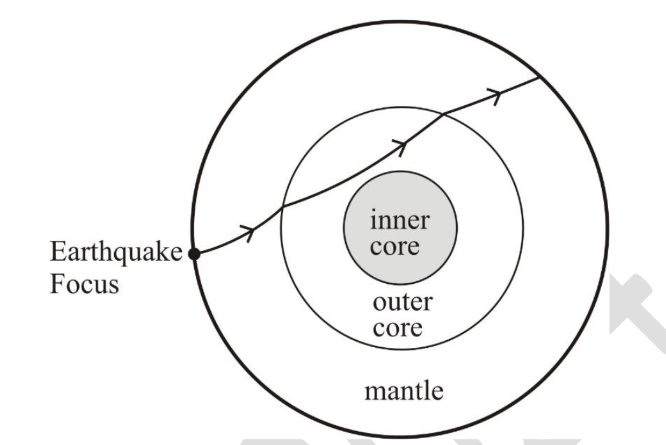
\includegraphics[width=0.4\textwidth]{figs/fig4.png}
    \caption{}
    \label{fig:q18}
\end{figure}


\hfill{\brak{\text{GATE GG 2024}}}

\begin{multicols}{4}
\begin{enumerate}
    \item PcP
    \item PKP
    \item PPP
    \item PmP
\end{enumerate}
\end{multicols}

\item Match the geophysical methods in Group–I with their associated physical properties in Group–II.
\begin{tabular}{ll}
\textbf{Group–I} & \textbf{Group–II} \\
P. Magnetic & 1. Chargeability \\
Q. Gravity & 2. Electrical conductivity \\
R. Magnetotelluric & 3. Susceptibility \\
S. Induced Polarization & 4. Density \\
\end{tabular}

\hfill{\brak{\text{GATE GG 2024}}}

\begin{enumerate}
    \item P-3, Q-4, R-2, S-1
    \item P-3, Q-4, R-1, S-2
    \item P-4, Q-3, R-2, S-1
    \item P-2, Q-1, R-4, S-3
\end{enumerate}
\newpage
\item The number of planes of symmetry in a tetrahedron is

\hfill{\brak{\text{GATE GG 2024}}}

\begin{multicols}{4}
\begin{enumerate}
    \item 9
    \item 6
    \item 4
    \item 3
\end{enumerate}
\end{multicols}


\item Which of the following Epochs belong(s) to the Quaternary Period?  

\hfill{\brak{\text{GATE GG 2024}}}

\begin{multicols}{2}
\begin{enumerate}
\item Holocene
\item Pleistocene
\item Pliocene
\item Miocene
\end{enumerate}
\end{multicols}

\item Which one or more of the following minerals shows O:Si ratio of 4:1 in its silicate structure?  

\hfill{\brak{\text{GATE GG 2024}}}

\begin{multicols}{2}
\begin{enumerate}
\item Olivine
\item Quartz
\item Diopside
\item Albite
\end{enumerate}
\end{multicols}

\item Which of the following rock structures is/are fold(s)?  

\hfill{\brak{\text{GATE GG 2024}}}

\begin{multicols}{2}
\begin{enumerate}
\item Antiform
\item Horst
\item Syncline
\item Synform
\end{enumerate}
\end{multicols}

\item Assume heat producing elements are uniformly distributed within a 16 km thick layer in the crust in a heat flow province. Given that the surface heat flow and reduced heat flow are 54 mW/m$^2$ and 22 mW/m$^2$, respectively, the radiogenic heat production in the given crustal layer in $\mu$W/m$^3$ is  (in integer).  

\hfill{\brak{\text{GATE GG 2024}}}

\item A confined aquifer with a uniform saturated thickness of 10 m has hydraulic conductivity of $10^{-2}$ cm/s. Considering a steady flow, the transmissivity of the aquifer in m$^2$/day is  (rounded off to one decimal place).  

\hfill{\brak{\text{GATE GG 2024}}}

\item A current of 2 A passes through a cylindrical rod with uniform cross-sectional area of 4 m$^2$ and resistivity of 100 $\Omega$-m. The magnitude of the electric field (E) measured along the length of the rod in V/m is  (in integer).  


\textbf{PART B2: FOR Geophysics CANDIDATES ONLY}


\item With increasing depth in the Earth, the P-wave velocity shows a significant decrease across which one of the following boundaries?  

\hfill{\brak{\text{GATE GG 2024}}}

\begin{multicols}{2}
\begin{enumerate}
\item crust -- mantle
\item mantle -- outer core
\item outer core -- inner core
\item upper mantle -- lower mantle
\end{enumerate}
\end{multicols}

\item The fold of a 2D seismic survey is defined as the maximum number of traces in which one of the following gathers?  

\hfill{\brak{\text{GATE GG 2024}}}

\begin{multicols}{2}
\begin{enumerate}
\item Common midpoint gather
\item Common offset gather
\item Common shot gather
\item Common receiver gather
\end{enumerate}
\end{multicols}

\item The Z-transform of the sequence \{1, 0, 1, 0, 1\} is  

\hfill{\brak{\text{GATE GG 2024}}}

\begin{multicols}{2}
\begin{enumerate}
\item $1 + Z^2 + Z^4$
\item $1 + Z + Z^2$
\item $Z + Z^3 + Z^5$
\item $Z + Z^2 + Z^3$
\end{enumerate}
\end{multicols}

\item Which one among the following events recorded in a land seismic reflection survey using vertical component geophones has the highest apparent slowness?  

\hfill{\brak{\text{GATE GG 2024}}}

\begin{multicols}{2}
\begin{enumerate}
\item Primary P-wave reflection
\item Direct wave
\item Head wave
\item Ground roll
\end{enumerate}
\end{multicols}

\item A GPR pulse is propagated into a non-magnetic medium comprising of a single layer underlain by a half space. If the dielectric constants for the top layer and the half-space are $\varepsilon_1$ and $\varepsilon_2$, respectively, the reflection coefficient at normal incidence is  

\hfill{\brak{\text{GATE GG 2024}}}

\begin{multicols}{2}
\begin{enumerate}
\item $\dfrac{\sqrt{\varepsilon_1} - \sqrt{\varepsilon_2}}{\sqrt{\varepsilon_1} + \sqrt{\varepsilon_2}}$
\item $\dfrac{\sqrt{\varepsilon_1} + \sqrt{\varepsilon_2}}{\sqrt{\varepsilon_1} - \sqrt{\varepsilon_2}}$
\item $\dfrac{\sqrt{\varepsilon_1}}{\sqrt{\varepsilon_1} + \sqrt{\varepsilon_2}}$
\item $\dfrac{\sqrt{\varepsilon_2}}{\sqrt{\varepsilon_1} + \sqrt{\varepsilon_2}}$
\end{enumerate}
\end{multicols}

\item The given figure shows the self-potential anomaly observed over a two dimensional thin sheet-type ore body whose strike is perpendicular to the plane of the paper. Which one of the following directions of polarization of the ore body leads to the given anomaly?  

\begin{figure}[h!]
    \centering
    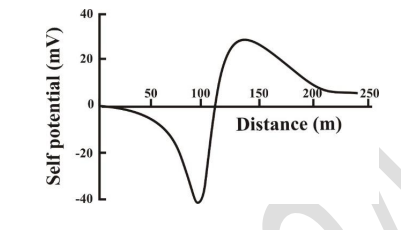
\includegraphics[width=0.4\textwidth]{figs/fig5.png}
    \caption{}
    \label{fig:q18}
\end{figure}


\hfill{\brak{\text{GATE GG 2024}}}


\begin{enumerate}
\item 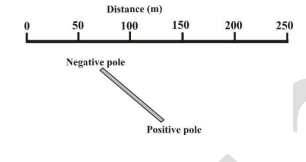
\includegraphics[width=0.4\textwidth]{figs/fig6.png}
\item 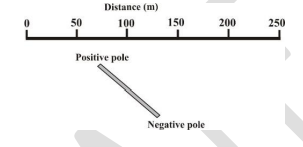
\includegraphics[width=0.4\textwidth]{figs/fig7.png}
\item 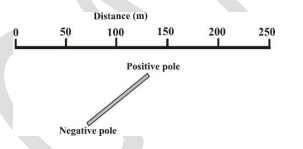
\includegraphics[width=0.4\textwidth]{figs/fig8.png}
\item 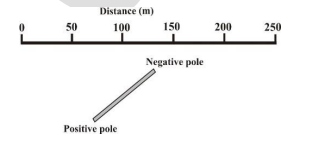
\includegraphics[width=0.4\textwidth]{figs/fig9.png}
\end{enumerate}


\item Which one of the following geophysical methods is suitable for the identification of seepage of water from dams?  

\hfill{\brak{\text{GATE GG 2024}}}

\begin{multicols}{2}
\begin{enumerate}
\item Self-Potential
\item Gravity
\item Magnetic
\item Radiometric
\end{enumerate}
\end{multicols}

\item The given beach-ball figure denotes the focal mechanism corresponding to which one of the following faults?  
\begin{figure}[h!]
    \centering
    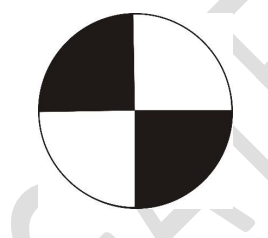
\includegraphics[width=0.4\textwidth]{figs/fig10.png}
    \caption{}
    \label{fig:q18}
\end{figure}


\hfill{\brak{\text{GATE GG 2024}}}

\begin{multicols}{2}
\begin{enumerate}
\item oblique slip normal
\item thrust
\item strike-slip
\item normal
\end{enumerate}
\end{multicols}

\item At present, which one of the following planets does NOT have a magnetic field of internal origin produced by an active dynamo?  

\hfill{\brak{\text{GATE GG 2024}}}

\begin{multicols}{2}
\begin{enumerate}
\item Mercury
\item Venus
\item Earth
\item Uranus
\end{enumerate}
\end{multicols}

\item The dimension of permeability is  

\hfill{\brak{\text{GATE GG 2024}}}

\begin{multicols}{2}
\begin{enumerate}
\item L
\item L$^2$
\item L$^3$
\item L$^2$T$^{-2}$
\end{enumerate}
\end{multicols}

\item In radiometric surveys, potassium in subsurface rocks will show a $\gamma$-ray peak in which one of the following MeV energy channels?  

\hfill{\brak{\text{GATE GG 2024}}}

\begin{multicols}{2}
\begin{enumerate}
\item 0.92
\item 1.46
\item 1.76
\item 2.62
\end{enumerate}
\end{multicols}

\item Assume the acceleration due to gravity is 10 m/s$^2$. The geoid height anomaly in metres due to the gravitational potential anomaly of $-59$ m$^2$/s$^2$ measured over the spheroid is  

\hfill{\brak{\text{GATE GG 2024}}}

\begin{multicols}{2}
\begin{enumerate}
\item -5.9
\item 5.9
\item 59
\item -59
\end{enumerate}
\end{multicols}

\item Which one among the following factors contributes the least amount of heat to the Earth’s annual heat budget?  

\hfill{\brak{\text{GATE GG 2024}}}

\begin{multicols}{2}
\begin{enumerate}
\item Geothermal flux from Earth’s interior
\item Reflection and re-radiation of Solar energy
\item Energy released from Earthquakes
\item Rotational deceleration by Tidal friction
\end{enumerate}
\end{multicols}

\item Identify the CORRECT assumption(s) supporting the convolutional model of zero-offset seismic data from the following statements.  

\hfill{\brak{\text{GATE GG 2024}}}


\begin{enumerate}
\item Seismic data consist of a single temporal frequency
\item There are no sharp changes in the material properties in the subsurface
\item Density is constant in the subsurface
\item The source waveform is stationary, that is, the source waveform does not change as it travels in the subsurface
\end{enumerate}



\item A spherical ore body produces a maximum gravity anomaly of 18 mGal when its centre is at a depth of 2 km from the surface. Assuming that the density contrast and the radius of the body remain unchanged, the ore body will produce a maximum gravity anomaly of 2 mGal if the depth to its centre in km is  \brak{\text{in integer}}.  

\hfill{\brak{\text{GATE GG 2024}}}

\item The ratio of the largest to the smallest amplitude of waveforms that can be accurately recorded by a digital seismometer is reported as $10^7$. Then, the dynamic range of the seismometer in dB is \brak{\text{in integer}}.  

\hfill{\brak{\text{GATE GG 2024}}}

\item A petroleum company estimates that a reservoir holds oil with a prior probability of 60\%. It then acquires petrophysical data that suggests the presence of oil. If the petrophysical analysis is accurate with a probability of 70\%, the posterior probability of the presence of oil in \% is  \brak{\text{rounded off to two decimal places}}.  

\hfill{\brak{\text{GATE GG 2024}}}

\item The magnitude of horizontal and vertical components of the total magnetic field at a particular location are 40500 nT and 36450 nT, respectively. The magnetic inclination at the same location in degrees is  \brak{\text{rounded off to one decimal place}}.  

\hfill{\brak{\text{GATE GG 2024}}}

\item A stress tensor $\boldsymbol{\sigma}$, with elements in MPa, is as given. The maximum value of the principal stress in MPa is
\[
\boldsymbol{\sigma}=\begin{bmatrix}
1 & 0 & \sqrt{2}\\
0 & 1 & 0\\
\sqrt{2} & 0 & 0
\end{bmatrix}
\]

\hfill{\brak{\text{GATE GG 2024}}}

\begin{multicols}{4}
\begin{enumerate}
\item 2.0
\item $\sqrt{2}$
\item 1.0
\item 0.0
\end{enumerate}
\end{multicols}

\item An overdetermined linear inverse problem is expressed as $\mathbf{G}\mathbf{m}=\mathbf{d}$, where $\mathbf{G}$ is the data kernel, $\mathbf{m}$ is the vector of model parameters and $\mathbf{d}$ is the vector of observed data. If damping is applied to the inverse problem and the resultant generalized inverse is represented by $\mathbf{G}^{-g}$, the model resolution matrix can be expressed as  

\hfill{\brak{\text{GATE GG 2024}}}

\begin{multicols}{2}
\begin{enumerate}
\item $\mathbf{G}^\mathrm{T}\mathbf{G}^{-g}$
\item $\mathbf{G}^{-g}\mathbf{G}^\mathrm{T}$
\item $\mathbf{G}^{-g}\mathbf{G}$
\item $\mathbf{G}\mathbf{G}^{-g}$
\end{enumerate}
\end{multicols}

\item A Wenner resistivity survey was performed with a spacing of 15 m between the current electrodes. Potential difference values of $-25$ mV and $225$ mV were measured before and after injecting 100 mA current into the ground. The apparent resistivity in $\Omega$-m after correcting for the self-potential effect is  

\hfill{\brak{\text{GATE GG 2024}}}

\begin{multicols}{4}
\begin{enumerate}
\item 78.5
\item 62.8
\item 188.5
\item 235.6
\end{enumerate}
\end{multicols}

\item Nine equally spaced electrodes are placed along a profile to perform Dipole–Dipole multi-electrode resistivity imaging. The maximum number of data points that can be obtained at measurement level $n=2$ is  

\hfill{\brak{\text{GATE GG 2024}}}

\begin{multicols}{4}
\begin{enumerate}
\item 5
\item 6
\item 4
\item 2
\end{enumerate}
\end{multicols}

\item Match the electromagnetic methods in Group–I with their corresponding frequency range in Group–II.  

\begin{tabular}{ll}
\textbf{Group–I} & \textbf{Group–II} \\
P. Very Low Frequency & 1.10 MHz –1 GHz \\
Q. Radio Magnetotelluric & 2.1 Hz – 20 kHz \\
R.Ground Penetrating Radar & 3.100 kHz – 1 MHz \\
S.Control Source Magnetotelluric & 4.15 kHz – 30 kHz \\
\end{tabular}  

\hfill{\brak{\text{GATE GG 2024}}}

\begin{multicols}{2}
\begin{enumerate}
\item P-4, Q-3, R-1, S-2
\item P-4, Q-3, R-2, S-1
\item P-2, Q-1, R-4, S-3
\item P-1, Q-2, R-3, S-4
\end{enumerate}
\end{multicols}

\item A geophysical forward problem is expressed as $d = 7m_1\,^{\!}2 m_2 + 6m_2$, where $m_1$ and $m_2$ represent the model parameters and $d$ represents the data. Then, the relationship between data and model parameters is  

\hfill{\brak{\text{GATE GG 2024}}}

\begin{multicols}{2}
\begin{enumerate}
\item explicit and linear
\item implicit and linear
\item explicit and non-linear
\item implicit and non-linear
\end{enumerate}
\end{multicols}

\item Assuming that the polar flattening of the Earth $f=3.353\times10^{-3}$, the difference between the geodetic and geocentric latitudes is maximum at  

\hfill{\brak{\text{GATE GG 2024}}}

\begin{multicols}{2}
\begin{enumerate}
\item the poles
\item $60^\circ$ geocentric latitude
\item $45^\circ$ geocentric latitude
\item $30^\circ$ geocentric latitude
\end{enumerate}
\end{multicols}

\item Which of the following statements related to an equipotential surface is/are CORRECT?  

\hfill{\brak{\text{GATE GG 2024}}}


\begin{enumerate}
\item Work is done on moving a test particle on an equipotential surface
\item Only one equipotential surface can exist at any point in space
\item The potential is constant on an equipotential surface
\item Field lines at any point are always parallel to their equipotential surface
\end{enumerate}


\item If $\mathbf{B}$ is the magnetic field in a region free of currents, then which of the following statements is/are correct?  

\hfill{\brak{\text{GATE GG 2024}}}

\begin{multicols}{2}
\begin{enumerate}
\item $\mathbf{B}=-\nabla\phi$, where $\phi$ is the scalar potential
\item $\mathbf{B}$ is rotational
\item $\nabla\times\mathbf{B}=\mathbf{0}$
\item $\nabla\cdot\mathbf{B}=\mathbf{0}$
\end{enumerate}
\end{multicols}

\item Which of the following operations performed in the time-domain with any two causal seismic signals result(s) in the subtraction of their corresponding phase spectra in the frequency domain?  

\hfill{\brak{\text{GATE GG 2024}}}

\begin{multicols}{2}
\begin{enumerate}
\item Convolution
\item Crosscorrelation
\item Deconvolution
\item Subtraction
\end{enumerate}
\end{multicols}

\item Choose the CORRECT statement(s) on the phenomenon of spatial aliasing of seismic data.  

\hfill{\brak{\text{GATE GG 2024}}}


\begin{enumerate}
\item Spatial aliasing can be reduced by increasing the geophone \brak{\text{group}} spacing
\item Spatial aliasing is more likely to occur for higher temporal frequencies in the data
\item Subsurface formations with higher interval velocities increase the likelihood of spatial aliasing
\item Reflections from steep dips are more likely to be spatially aliased
\end{enumerate}


\item The speed of a ship is given as $V_1$ and $V_2$ in km/h and knots, respectively. The latitude of observation and the direction of the ship with respect to the North are represented as $\theta_1$ and $\theta_2$, respectively. The CORRECT expression(s) for the E\"otv\"os correction in mGal is/are  

\hfill{\brak{\text{GATE GG 2024}}}

\begin{multicols}{1}
\begin{enumerate}
\item $4.040\,V_1\cos\theta_1\sin\theta_2+0.001211\,V_1^2$
\item $7.503\,V_2\cos\theta_1\sin\theta_2+0.004154\,V_2^2$
\item $4.040\,V_2\cos\theta_2\sin\theta_1+0.001211\,V_2^2$
\item $7.503\,V_1\cos\theta_1\sin\theta_2+0.004154\,V_1^2$
\end{enumerate}
\end{multicols}

\newpage

\item Which of the following statements pertaining to the interpretation of Neutron log is/are CORRECT?  

\hfill{\brak{\text{GATE GG 2024}}}


\begin{enumerate}
\item Overpressured shale shows very low neutron porosity
\item Neutron log primarily measures liquid \brak{\text{water/oil}} filled porosity
\item Neutron porosity for a gas-bearing clean sandstone formation is lower than the actual porosity of the same formation
\item A low neutron porosity indicates high Hydrogen Index of the formation
\end{enumerate}


\item A magnetic field \brak{\text{B}} of strength 50000 nT induces a magnetization \brak{\text{M}} of magnitude 5 A/m in a rock. Given the magnetic permeability of free space $\mu_0=4\pi\times10^{-7}$ H/m, the susceptibility of the rock is\brak{\text{rounded off to three decimal places}}.  

\hfill{\brak{\text{GATE GG 2024}}}

\item The amplitude of a monochromatic 1000 Hz EM wave reduces by a factor of $1/e$ after penetrating to a depth of 100 m in a homogeneous medium. Given the magnetic permeability of free space $\mu_0=4\pi\times10^{-7}$ H/m, the electrical conductivity of the medium in S/m is \brak{\text{rounded off to three decimal places}}.  

\hfill{\brak{\text{GATE GG 2024}}}

\item A plane P-wave is incident at an angle of $60^\circ$ with respect to the normal to a horizontal reflector. If the incident medium is a homogeneous Poisson solid \brak{\text{Poisson’s ratio of 0.25}}, the angle of the reflected, mode-converted S-wave in degrees with respect to the normal is   \brak{\text{rounded off to one decimal place}}.  

\hfill{\brak{\text{GATE GG 2024}}}

\item A marine seismic survey was performed in a region with a flat, horizontal sea bed at a depth of 100 m from the sea surface. The datum of the stacked seismic section was fixed at the sea surface. If the P-wave velocity in water is 1600 m/s, the radius of the first Fresnel zone at the sea bed at a frequency of 50 Hz corresponding to the stacked seismic section is  \brak{\text{rounded off to one decimal place}}.  

\hfill{\brak{\text{GATE GG 2024}}}

\item A stacked seismic section shows a single dipping event with a slope of 0.5 s/km. Stolt migration with a constant velocity of 2 km/s is applied to the data. The dip of the event in the migrated section in degrees is  \brak{\text{rounded off to one decimal place}}.  

\hfill{\brak{\text{GATE GG 2024}}}

\item The number of half-lives \brak{\text{$t_{1/2}$}} required for a radioactive isotope to decrease to 2\% of its original abundance is  \brak{\text{rounded off to two decimal places}}.  

\hfill{\brak{\text{GATE GG 2024}}}

\item A monochromatic cosine wave with frequency of 0.24 Hz and wavelength 16 km interferes with another monochromatic cosine wave with frequency 0.3 Hz and wavelength 10 km. The group velocity of the resulting wave in km/s is \brak{\text{rounded off to one decimal place}}.  

\hfill{\brak{\text{GATE GG 2024}}}

\newpage

\item The given figure shows a homogeneous rock layer of thickness 100 m. A vertical borehole is drilled through the rock layer and gravity measurements are acquired at points A and B. If the difference in measurements at A and B is 5 mGal, the density of the rock layer \brak{\text{$\rho$}} in g/cc, ignoring terrain corrections is \brak{\text{rounded off to two decimal places}}.  

\begin{figure}[h!]
    \centering
    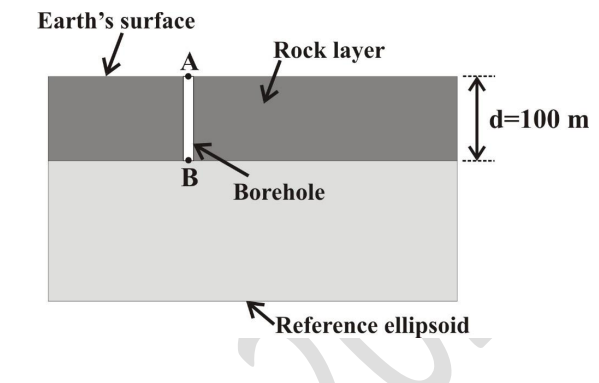
\includegraphics[width=0.4\textwidth]{figs/fig11.png}
    \caption{}
    \label{fig:q18}
\end{figure}


\hfill{\brak{\text{GATE GG 2024}}}





\end{enumerate}


\begin{align*}
 {\LARGE{\textbf{END OF THE QUESTION PAPER}}}
\end{align*}


\end{document}
